% You should title the file with a .tex extension (hw1.tex, for example)
\documentclass[a4paper, 11pt]{article}

\usepackage{amsmath}
\usepackage{amssymb}
\usepackage{fancyhdr}
\usepackage{graphicx}
\usepackage{fancyvrb}
\usepackage[margin=1in]{geometry}
\usepackage{hyperref}
\usepackage{graphicx}
\graphicspath{ {./images/} }
\usepackage[export]{adjustbox}
\usepackage{placeins}

\newcommand{\question}[2] {\vspace{.25in} \hrule\vspace{0.5em}
\noindent{\bf #1: #2} \vspace{0.5em}
\hrule \vspace{.10in}}
\renewcommand{\part}[1] {\vspace{.10in} {\bf (#1)}}

\newcommand{\myname}{Chakeera W, Sirin C, Natthakan E.}
\newcommand{\myemail}{}
\newcommand{\myhwnum}{5}

\setlength{\parindent}{0pt}
\setlength{\parskip}{5pt plus 1pt}
 
\pagestyle{fancyplain}
\lhead{\fancyplain{}{\textbf{Population Estimation}}}      % Note the different brackets!
\rhead{\fancyplain{}{\myname}}
\chead{\fancyplain{}{ICCS240}}

\begin{document}

\medskip                        % Skip a "medium" amount of space
                                % (latex determines what medium is)
                                % Also try: \bigskip, \littleskip

\thispagestyle{plain}
\begin{center}                  % Center the following lines
{\Large ICCS240: Database Project} \\
{\Large Population Estimation in Thailand} \\
21 March 2020
\end{center}
\question{Group Members}

Sirin Chankao (5980753)\\
Chakeera Wansoh (6080566)\\
Natthakan Euaumpon (6081213)\\

\question{Note to Professor}

Due to the current situation, we got limited time but we really want to complete this project so even after we submit this project today (21-03-2020) we will continue to work on it therefore, there will be constant update in our github site until the last final date of submission (i.e, 29-03-2020)\\
\question{Overview}

This project use the different concepts of database management system and linear algebra. From linear algebra, we learned that eigenvector can be use to estimate the population with this idea in mind we decided to combine this with our DBMS knowledge. Therefore, the aim of this project is to estimate the future population of regions in Thailand by calculating from the previous years. Many of the project's informations (or evidences that the database exists) can be seen in the project's github. \url{https://github.com/chakeera/PopulationEstimation} \\
\question{Theory}

 For the sake of explanation, let assume that A is a matrix. This will work only if A is a symmetric matrix. We need to find all positive eigenvalues which are required for our numerical approach. We are going to implement this by combining Power Method with Rayleigh quotient iteration. This iteration has the following formula:
 \begin{center}
     $b_{i+1} = \frac{(A-\mu_{i}I)^{-1}b_{i}}{||(A-\mu_{i}I)^{-1}b_{i}||} $ 
 \end{center}
Where $b_{i+1}$ is the next approximation of the eigenvector and \italic{I} is the identity matrix. After that we can set the next approximation of an eigenvalue to the Rayleigh quotient:
 \begin{center}
$\mu_{i+1} = \frac{b^{*}_{i+1}Ab_{i+1}}{b^{*}_{i+1}b_{i+1}}$
 \end{center}
However, we need to compute all eigenvalues so we need to combine this technique with a deflation technique. Now we will get the largest possible eigenvalue. But we need to consider all of them. There are many deflation methods, but for this project, we are going to use Hotelling’s deflation. This is one of the most popular techniques.
 \begin{center}
$(A-\lambda_{1}u_{1}u_{1}^{T})$
\end{center}
Where \italic{u} is elements in a set of N vectors, as eigenvectors are the set of N vectors of A. From the equation above, we will get the matrix that has the same eigenvectors and eigenvalues as matrix A. But the largest eigenvalue is replaced with 0. Thus we can combine this with power method and Rayleigh quotient to find the next biggest and so on until we find all the eigenvalues. Then we substitute the eigenvalues into a matrix to get our eigenvectors where it will be multiplied with \italic{nxn} matrix that is the matrix of the offsprings and number of survivors and its result will give us the estimated population value.\\

\question{Database schema}

We have total three tables in our database with the following schema:\\
(These tables import data from "dataset" folder in github)
\begin{Verbatim}[commandchars=+\[\]]
    AgeStructure(Year INT, Age TEXT, Percentage NUMERIC)
    
    RegionPopulation(Region TEXT, Year INT, Population NUMERIC)
    
    TotalPopulation(+underline[Year] INT, Population NUMERIC, Yearly_percent_change NUMERIC, 
    Yearly_change NUMERIC, Migrants INT,Median_Age NUMERIC, 
    Fertility_Rate NUMERIC, Density INT, Urban_percent NUMERIC,
    Urban_Population NUMERIC, Country_Share NUMERIC,Global_Rank INT)
\end{Verbatim}

\question{Backend}

For back end, we select values from database and insert them into a $6*6$ matrix. This is done by creating a function called "getValueX" and "getValueY". Let x be a fraction of the change in population in each year and y be the total number of offspring produced each year. Lets $x_1$ and $y_1$ be the value for the first year and so on. Then we would get a matrix that look like:\\
\begin{figure}[h]
    \centering
\begin{bmatrix}
0 & $y_2$ & $y_3$ & $y_4$ & $y_5$ & $y_6$\\
$x_1$ & 0 & 0 & 0 & 0 & 0\\
0 & $x_2$ & 0 & 0 & 0 & 0\\
0 & 0 & $x_3$ & 0 & 0 & 0\\
0 & 0 & 0 & $x_4$ & 0 & 0\\
0 & 0 & 0 & 0 & $x_5$ & 0
\end{bmatrix}
\end{figure}

We will put this in form of nested 2D array. Where each sub-array will contain values in each row. After that we compute eigenvalues. For this project, we only want a positive eigenvalues. This is done by using power method, Rayleigh quotient, LU decomposition and deflation techniques. We, then, convert a matrix from above function to matrix form and compute. We will continue doing until we get a satisfied values. Then we compute eigenvector. Which will then be multiplied with a original given matrix that we retrieved from a database to get our final results. Our final results would be an array that each values is the approximation of the total population in each age group.\\

\question{Frontend}

For front end, we use Java GUI to present our resulting data. There will be mainly three windows. The first window as shown in the first figure below. This window will act as the menu window where user can select which option they wanted to use. The option includes 'Population in Thailand' and 'Estimation of  Population.' If the user selects 'Population in Thailand,' the 'Population in Thailand' window will appear as shown in the second figure below. If the user selects 'Estimation of  Population,' the 'Estimation of  Population' window will appear as shown in the third figure below. 

\begin{figure}[h]
    \centering
    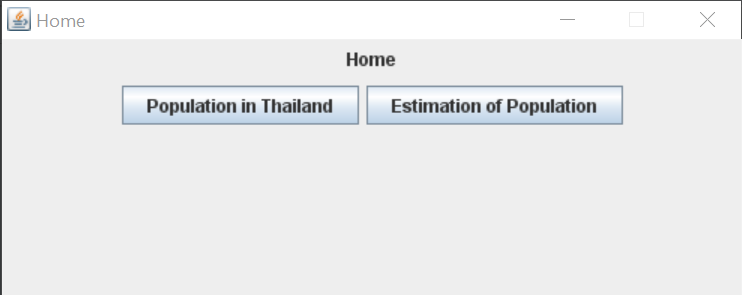
\includegraphics[scale=0.75, center]{GUI Home.png}
    \caption{Home Window}
\end{figure}
\begin{figure}[h]
    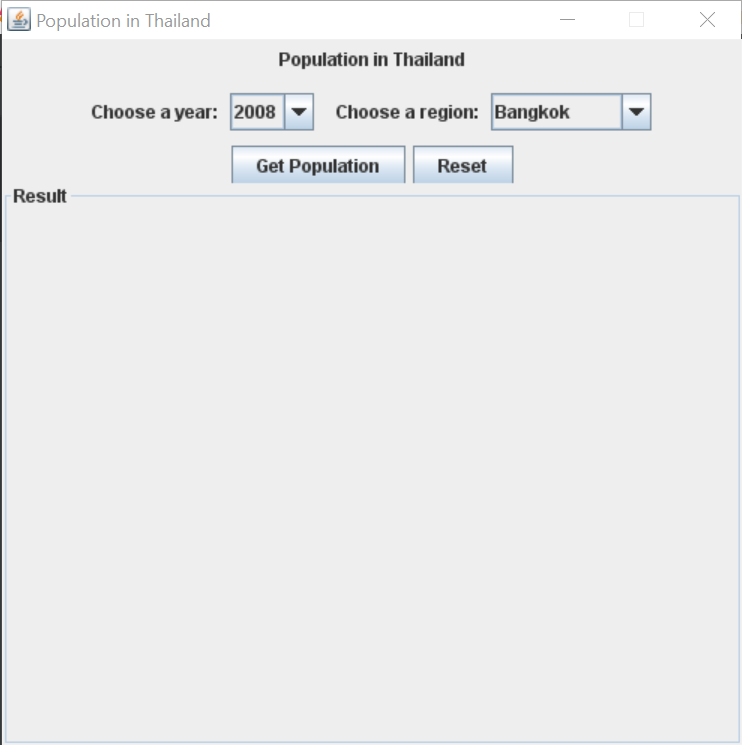
\includegraphics[scale=0.75, center]{GUI CurPop.png}
    \caption{Current Population Window}
\end{figure}
\begin{figure}[h]
    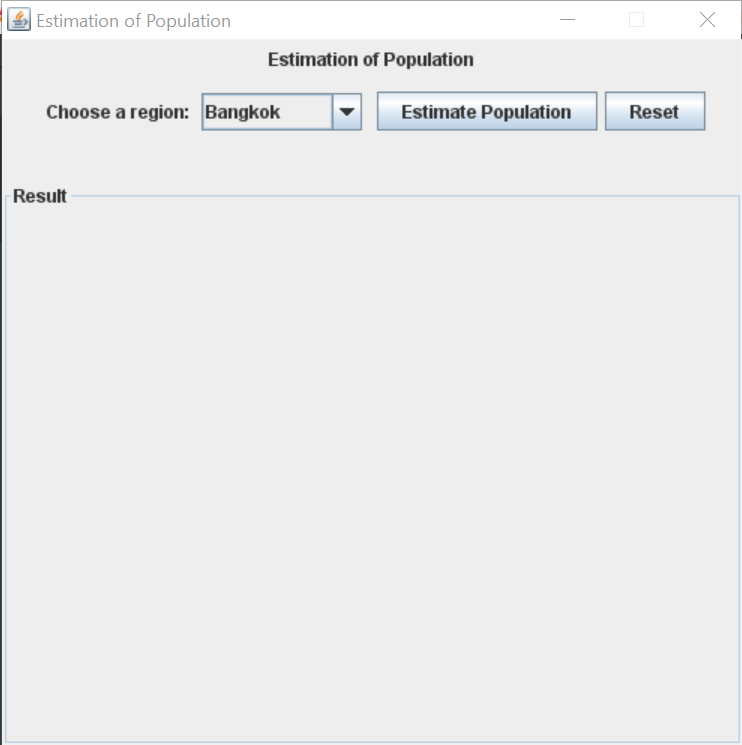
\includegraphics[scale=0.75, center]{GUI EstPop.png}
    \caption{Estimation Window}
\end{figure}
\FloatBarrier

\question{Video}

Video will be post in github under the folder "Report and Video"\\

\question{Unfinished functions}

\begin{itemize}
\item Linking the postgres database with intelliJ to compute the matrix function.\\
\item Finish getValueX() and getValueY() functions.\\
\item Present the resulting data in the front end after computing matrix function.\\
\item Making video

\end{itemize}


\end{document}


